\documentclass[10pt]{article}
\usepackage[utf8]{inputenc}
\usepackage[T1]{fontenc}
\usepackage{amsmath}
\usepackage{amsfonts}
\usepackage{amssymb}
\usepackage[version=4]{mhchem}
\usepackage{stmaryrd}
\usepackage{hyperref}
\usepackage{graphicx}
\usepackage{enumitem}
\usepackage{multirow}
\graphicspath{ {./CS-234/} }

\title{Assignment 3 - Quantifiers, Asymptotics, and NFAs}

\author{CS 234}
\date{Daniel Lee}


\begin{document}
\maketitle

\section*{1 \quad Quantifiers and NFAs on Paper}

\begin{enumerate}[label={}]
      \item Write the following as English statements with no mathematical notation.


            3.47. $\forall n \in \mathbb{N}, 2 n \in \mathbb{N}$

            For all natural number $n$, two times $n$ is also a natural number.\\


            3.50. $\forall n \in \mathbb{Z}, \exists m \in Z, m<n$

            For all integer $n$, there exists an integer $m$ such that $m$ is smaller than $n$.\\


            3.52. $\forall n \in \mathbb{N}, \exists s \in\{0,1\}^*,|s|=n$

            For all natural number $n$, there exists a string $s$ that is in the set of all strings formed by 0s or 1s or both 0s and 1s or the empty string such that the length of string $s$ is $n$.\\


            3.53. $\forall s \in\{0,1\}^*, \exists q, r \in\{0,1\}^*, s=q r$

            For all string $s$ that is in the set of all strings formed by 0s or 1s or both 0s and 1s or the empty string, there exist strings $q$ and $r$ that are in the set of all strings formed by 0s or 1s or both 0s and 1s or the empty string such that string $s$ is equivalent with string $qr$.\\


      \item Show the following Big-O relationships by giving constants $c$ and $n_0$ in each case and showing that they work.


            3.55. $7 n-2 \in O(n)$

            The function $f(n)=7 n-2$ is $O(n)$ using $c=8$ and $n_0=4$, that is, $7 n-2 \leq 8 n$ for all $n \geq 4$. This is true because $-2 \leq n$ for all $n \geq 4$, so $7 n-2 \leq 7 n+n=8 n$ for all $n \geq 4$.\\


            3.56. $2 n^2+4 \in O\left(n^2\right)$

            The function $f(n)=2 n^2+4$ is $O\left(n^2\right)$ using $c=6$ and $n_0=1$, that is, $2 n^2+4 \leq 6 n^2$ for all $n \geq 1$. This is true because $4 \leq 4 n^2$ for all $n \geq 1$, so $2 n^2+4 \leq 2n^2+4 n^2=6 n^2$ for all $n \geq 1$.\\

            3.57. $3 n^2-2 n+4 \in O\left(n^2\right)$

            The function $f(n)=3 n^2-2 n+4$ is $O\left(n^2\right)$ using $c=9$ and $n_0=1$, that is, $3 n^2-2 n+4 \leq 9 n^2$ for all $n \geq 1$. This is true because $-2 n \leq 2 n^2$ for all $n \geq 1$ and $4 \leq 4 n^2$ for all $n \geq 1$, so $3 n^2-2 n+4 \leq 3n^2+2 n^2 + 4 n^2=9 n^2$ for all $n \geq 1$.\\


            3.58. $n^3-n^2+n-1 \in O\left(n^3\right)$

            The function $f(n)=n^3-n^2+n-1$ is $O\left(n^3\right)$ using $c=4$ and $n_0=1$, that is, $n^3-n^2+n-1 \leq 4 n^3$ for all $n \geq 1$. This is true because $-n ^2 \leq n^3$ for all $n \geq 1$, $n \leq n^3$ for all $n \geq 1$, and $-1 \leq n^3$ for all $n \geq 1$, so $n^3-n^2+n-1 \leq n^3 + n^3 + n^3 + n^3=4 n^3$ for all $n \geq 1$.\\


      \item Negate the following quantified statements.


            3.65. $\forall n \in \mathbb{R}, 2 n \in \mathbb{R}$


            $\exists n \in \mathbb{R}, 2 n \notin \mathbb{R}$

            3.69. $\forall n \in \mathbb{N}, \exists s \in\{0,1\}^*,|s|=n$

            $\exists n \in \mathbb{N}, \forall s \in\{0,1\}^*, |s|\neq  n$

            3.71.$\exists w \in \Sigma^*, \forall x, y \in \Sigma^*, \exists z \in \Sigma^*,(|w x| \leq|y z|) \vee(|z x| \leq|y w|)$

            $\forall w \in \Sigma^*, \exists x, y \in \Sigma^*, \forall z \in \Sigma^*,(|w x| > |y z|) \wedge  (|z x| > |y w|)$


      \item Give a sequence of states that show that the following strings are accepted by the following NFAs:

            4.5. 101010 for the NFA in Example 4.6

            $q_0$ → $q_2$ → $q_3$ → $q_2$ → $q_3$ → $q_2$ → $q_3$

            4.7. baaab for the NFA in Example 4.8

            $q_0$ → $q_0$ → $q_0$ → $q_0$ → $q_1$ → $q_2$


      \item Draw nondeterministic finite automata (that are not also deterministic ones) with no $\lambda$ transitions for the following languages:

            4.8. $\left\{w \in\{0,1\}^*: w\right.$ ends in 00$\}$

            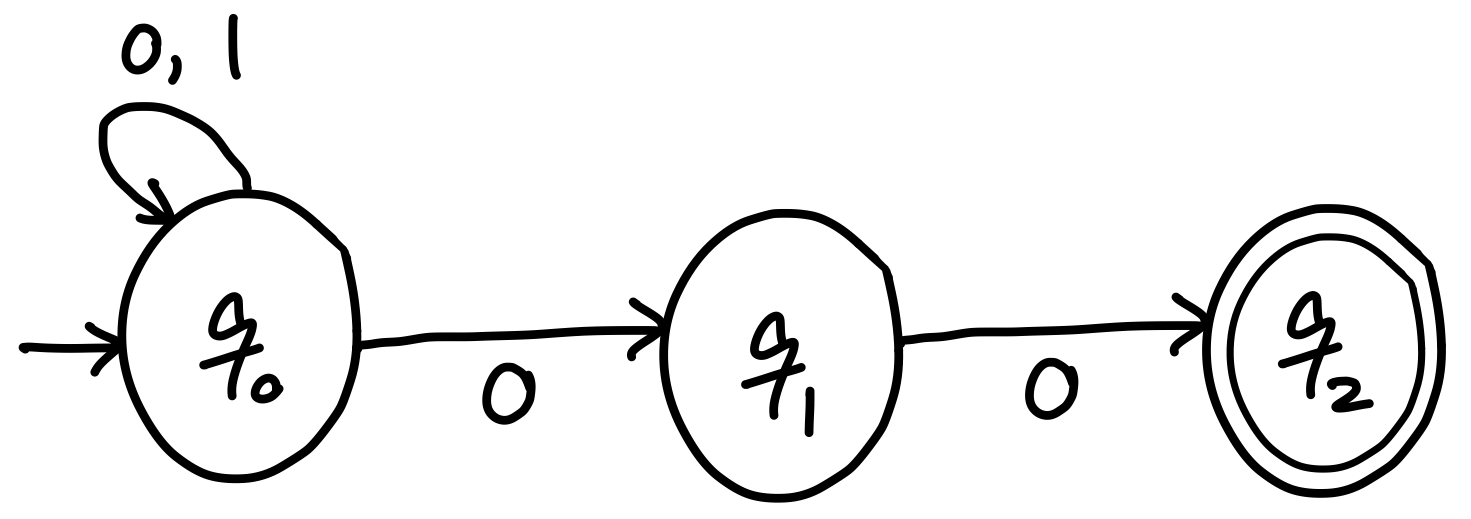
\includegraphics[scale=0.3]{4.8}


            4.10. $\left\{w \in\{0,1\}^*: w\right.$ has 01 or 10 as a substring $\}$

            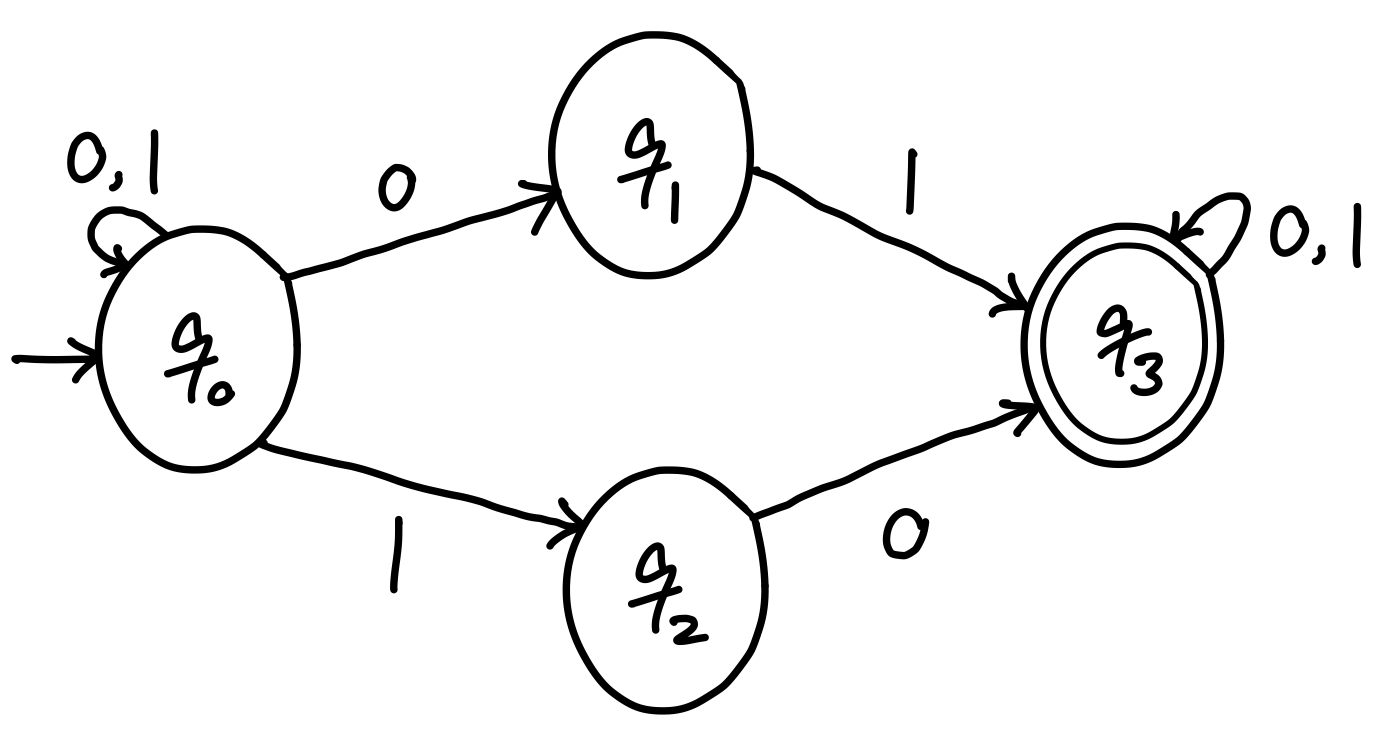
\includegraphics[scale=0.3]{4.10}


            4.13. $\left\{w \in\{0,1\}^*: w\right.$ starts with 00 and ends with 11$\}$

            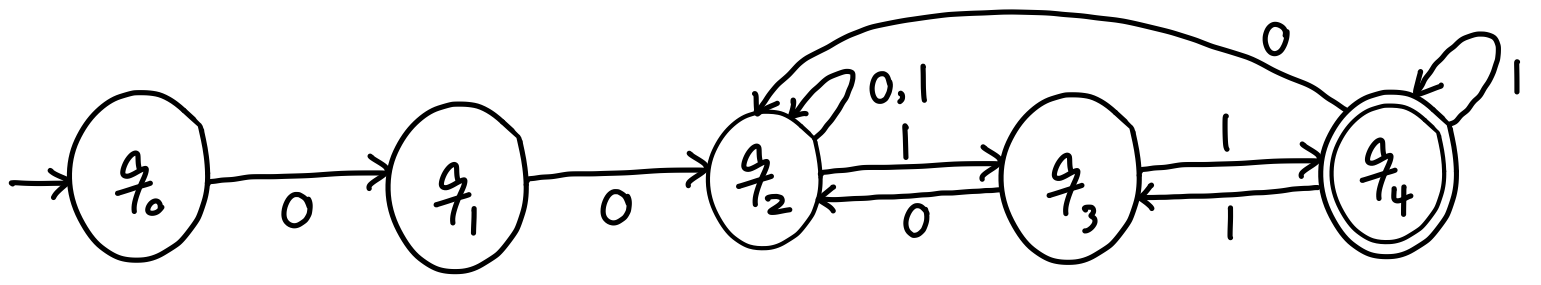
\includegraphics[scale=0.3]{4.13}


            4.14. $\{a\}^* \cup\left\{(a b)^n: n \geq 1\right\}$

            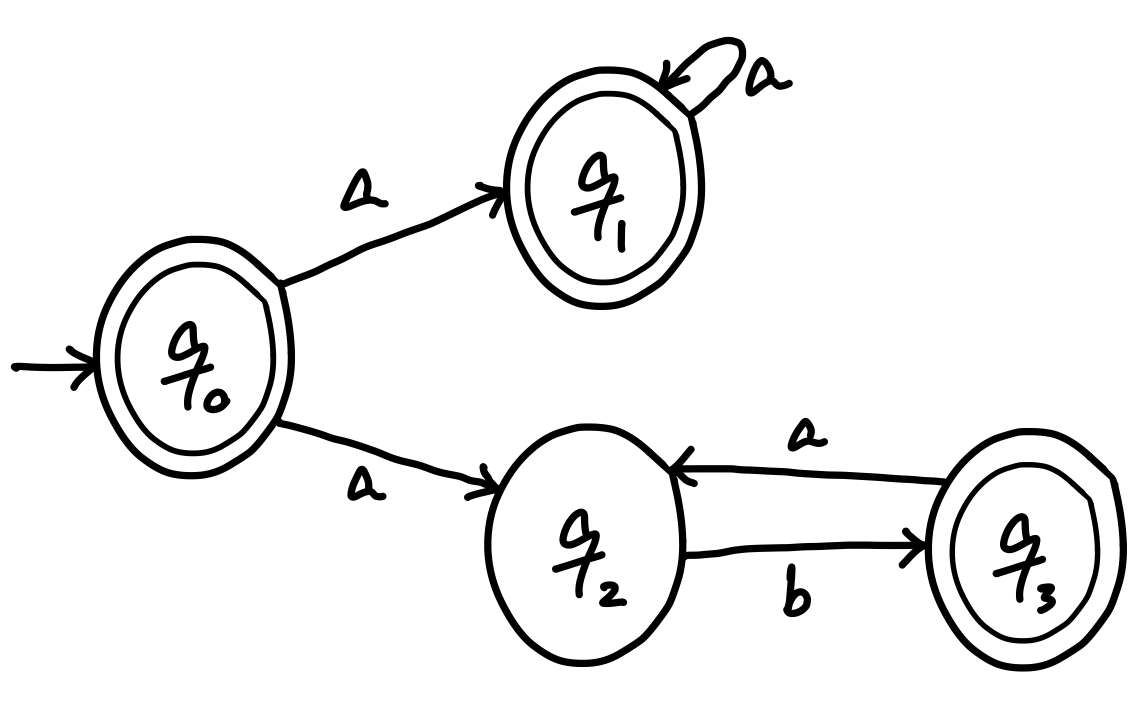
\includegraphics[scale=0.3]{4.14}


            4.16. $\left\{0^p 1^q 0^r: p \geq 1, q \geq 0, r \geq 1\right\}$

            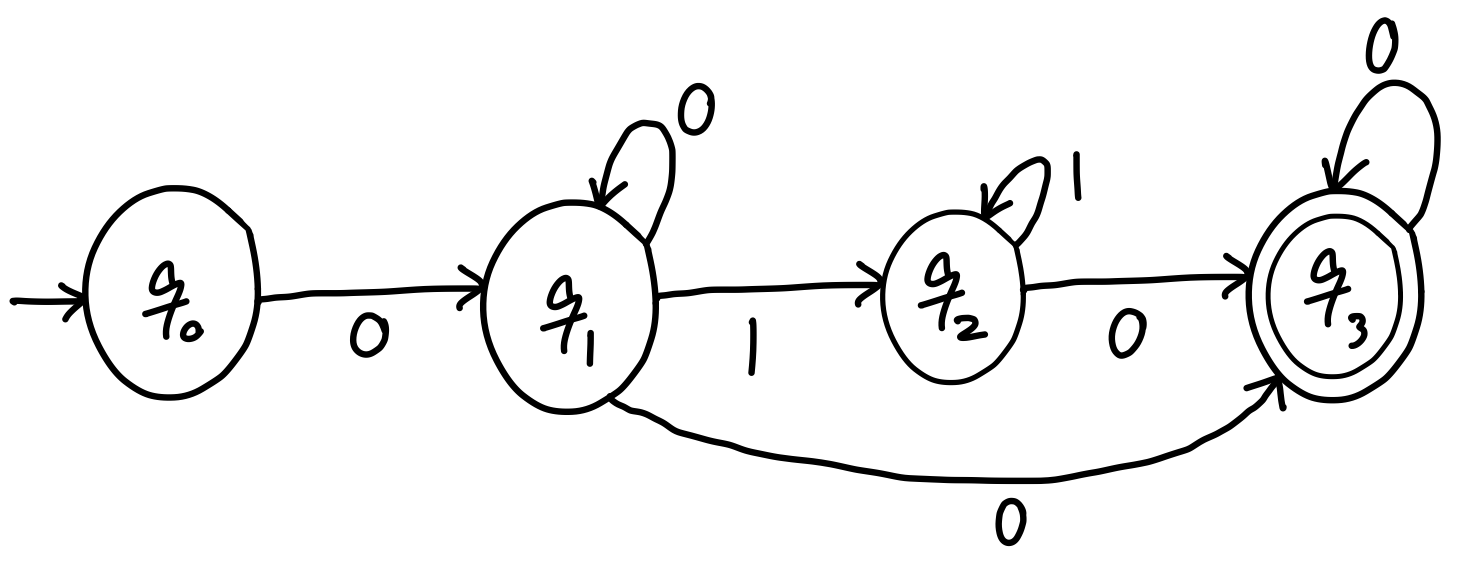
\includegraphics[scale=0.3]{4.16}

            4.18. $\left\{w \in\{0,1\}^*:\right.$ at least one of the last three characters from the end is a 0$\}$

            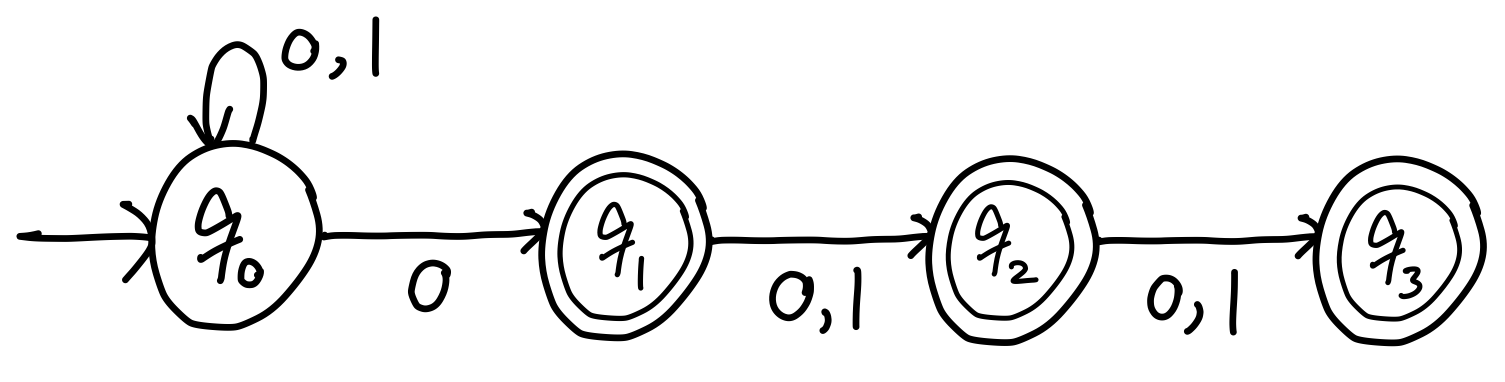
\includegraphics[scale=0.3]{4.18}

            4.19. $\left\{w \in\{0,1\}^*: w\right.$ does not have 01 as a substring $\}$

            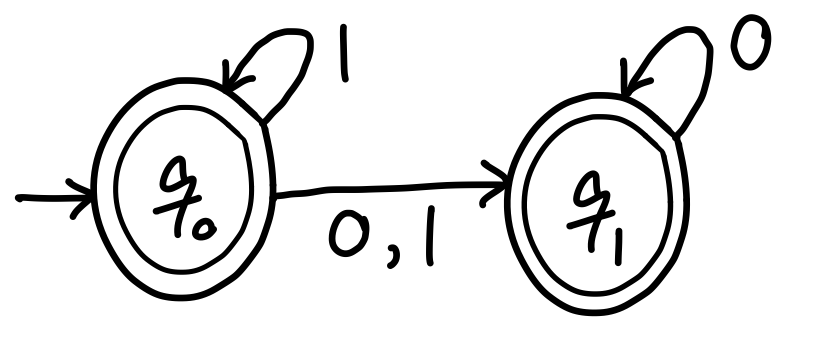
\includegraphics[scale=0.3]{4.19}


      \item Convert the following NFAs to DFAs using the Subset Construction algorithm:


            4.20. The NFA in Example 4.4

            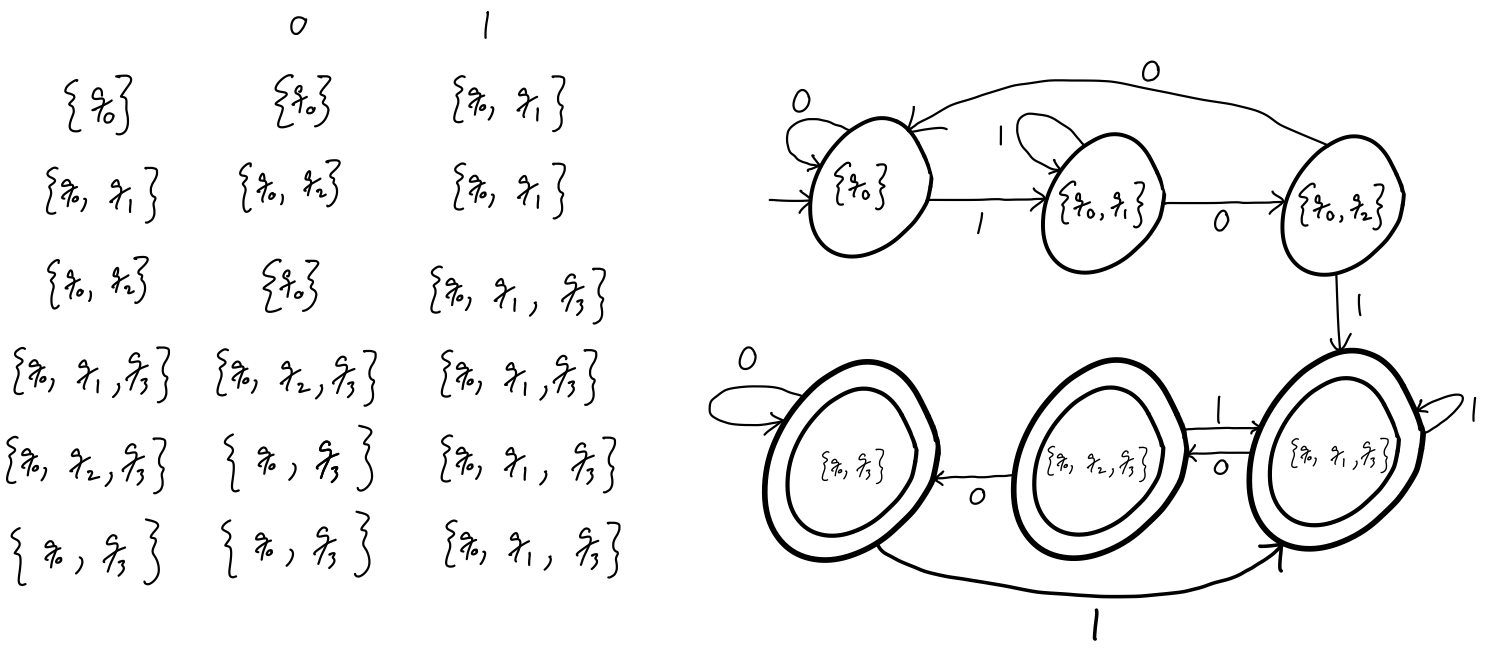
\includegraphics[scale=0.5]{4.20}

            4.22. The NFA in Example 4.8

            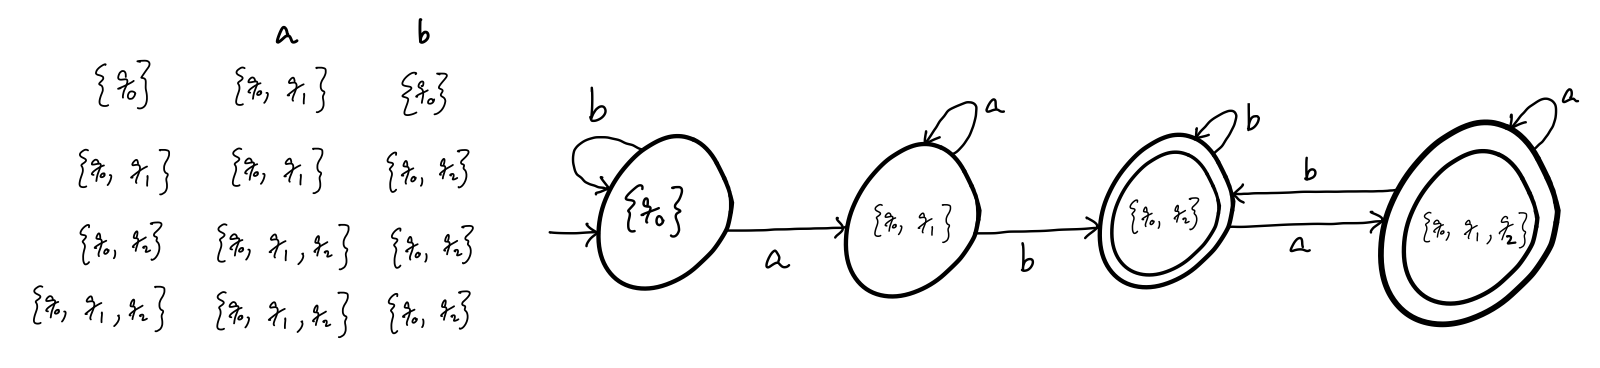
\includegraphics[scale=0.5]{4.22}





\end{enumerate}

\end{document}